\title{Algèbre Linéaire Numérique}

\vspace{-6em}{
	\tiny
	\hfill
	prière de bien vouloir envoyer des corrections/commentaires à
	\tt enric.meinhardt@ens-paris-saclay.fr
}\vspace{3em}

\newcommand{\ds}{\displaystyle}

\newcommand{\1}{\mathbf{1}}
\newcommand{\N}{\mathbf{N}}
\newcommand{\Z}{\mathbf{Z}}
\newcommand{\Q}{\mathbf{Q}}
\newcommand{\R}{\mathbf{R}}
\newcommand{\C}{\mathbf{C}}
\newcommand{\K}{\mathbf{K}}
\newcommand{\T}{\mathbf{T}}
\newcommand{\M}{\mathbf{M}}
\newcommand{\ud}{\mathrm{d}}
\newcommand{\e}{\mathbf{e}}
\newcommand{\x}{\mathbf{x}}
\newcommand{\y}{\mathbf{y}}
\newcommand{\z}{\mathbf{z}}
\newcommand{\Sp}{\mathrm{Sp}}
%\renewcommand{\Re}{\operatorname{Re}}
%\renewcommand{\Im}{\operatorname{Im}}
\newcommand{\OO}{\mathcal{O}}

\newcommand{\parens}[1]{\left(#1\right)} % (x)
\newcommand{\pairing}[2]{\left\langle #1,#2\right\rangle} % <x,y>

% \abs{x}   ->    |x|
% \Abs{x}   ->   ||x||
% \ABS{x}   ->  |||x|||
\newcommand{\abs}[1]{\left|#1\right|}
\newcommand{\Abs}[1]{\left\|#1\right\|}
\newcommand{\ABS}[1]{{\left\vert\kern-0.25ex\left\vert\kern-0.25ex\left\vert #1 \right\vert\kern-0.25ex\right\vert\kern-0.25ex\right\vert}}



\section{Introduction}

L'objectif de ces notes est d'expliquer les méthodes principales de
\emph{résolution d'un système linéaire} et de~\emph{calcul d'éléments
propres} d'une matrice.  Pour la résolution de systèmes, il y a deux types de
méthodes.  Les~\emph{méthodes directes} construisent le vecteur solution en
faisant un nombre fini d'opérations arithmétiques sur les données d'entrée
qui amènent à la solution exacte.  Les \emph{méthodes itératives}, trouvent
une suite de vecteurs qui converge vers le vecteur solution.  Pour le calcul
des éléments propres, toutes les méthodes en dimension~$\ge 5$ sont
nécessairement itératives.

Afin d'évaluer la performance de ces méthodes, nous introduisons les éléments
de base de l'analyse matricielle.
Nous proposons aussi plusieurs exemples d'application.

{\small\sl Ces notes sont basées partiellement sur un poly antérieur de Lionel
Magnis.}

\subsection{Références}

[AK]
G.~Allaire et S.~M.~Kaber,
\emph{Algèbre linéaire numérique}.
Ellipses 2002.

%	[All]
%		G.~Allaire,
%		\emph{Analyse numérique et optimisation}.
%		Éditions de l'École Polytechnique, 2005.

[Cia]
P.~G.~Ciarlet,
\emph{Introduction à l'analyse numérique matricielle et à
l'optimisation}.
Masson, 1994.

[CH]
R.~Courant und D.~Hilbert,
\emph{Mathematische Physik}.
Springer 1931

[Ser]
D.~Serre,
\emph{Matrices: theory and applications}.
Springer, 2002.\\
Théorie générale des matrices avec un langage moderne.

%[Stra]
%G.~Strang,
%\emph{Introduction to applied mathematics}.
%Wellesley, 1986\\
%Collection énorme et très variée de modèles linéaires.

[W]
H.~Weyl,
\emph{The Classical Groups}.
Princeton University Press, 1939\\
Étude détaillée des sous-groupes du groupe linéaire général.

\clearpage
\subsection{Notations}

\begin{itemize}
	\item $\K$ est le corps~$\R$ ou~$\C$.
	\item $\pairing{\cdot}{\cdot}$ est le produit hermitien
		(si~$\K=\C$) ou scalaire (si~$\K=\R$) sur~$\K^n$.
		%On a donc~$\pairing{\x}{\y}=\sum_i x_i\overline y_i$.
	\item $\M_{p,q}(\K)$ est l'ensemble des matrices sur~$\K$
		avec~$p$ lignes et~$q$ colonnes.
		%Cet ensemble s'identifie de façon
		%naturelle avec les applications linéaires~$\K^p\to\K^q$.
	\item $\M_p(\K)$ est l'ensemble~$\M_{p,p}(\K)$ des matrices carrées.
	\item $A^*$ est la matrice conjuguée de~$A$ (si~$\K=\C$) ou transposée
		(si~$\K=\R$).
		%On a donc~$\parens{A^*}_{ij}=\overline{\parens{A}_{ji}}$.
	\item $GL_n(\K)$ est
	%~\emph{sa majesté le groupe linéaire général},
		l'ensemble des matrices inversibles de taille~$n$.
	\item $O_n(\R)$ est 
		%le~\emph{groupe orthogonal}
		l'ensemble des matrices orthogonales ($A^\top A=I$).
	\item $SO_n(\R)$ est
		%le~\emph{groupe unitaire spécial}
		l'ensemble des matrices orthogonales de déterminant~$1$.
	\item $U_n(\C)$ est
		%le~\emph{groupe unitaire}
		l'ensemble des matrices unitaires ($A^*A=I$).
	\item $SU_n(\C)$ est
		%le~\emph{groupe unitaire spécial}
		l'ensemble des matrices unitaires de déterminant~$1$.
	\item $TS_n(\K)$ (resp.~$TI_n(\K)$) est l'ensemble des matrices
		triangulaires supérieures (resp.~inférieures) de taille~$n$.
	\item $TS^{++}_n(\K)$ (et~$TI^{++}_n(\K)$) est l'ensemble des matrices
		triangulaires dont les éléments diagonaux sont strictement positifs.
	\item $TS^{1}_n(\K)$ (et~$TI^{1}_n(\K)$) est l'ensemble des matrices
		triangulaires dont les éléments diagonaux sont tous~$1$.
	\item $S_n(\R)$ (resp.~$H_n(\C)$) est l'ensemble des matrices
			symétriques~(resp.~hermitiennes), définies par la
			condition~$A^\top=A$ (resp.~$A^*=A$)
	\item $S^{++}_n(\R)$ (resp.~$H^{++}_n(\C)$) est l'ensemble des matrices
			symétriques définies positives~(resp.~hermitiennes définies positives),
		\item $\Sp_\C(A)=\left\{\lambda\in\C\ :\ \exists\x\in\K^n\ :\
			A\x=\lambda\x\right\}$ est le~\emph{spectre} de
			$A\in\M_n(\K)$.
	\item $\Abs{\x}_p$ est la norme~$p$ de~$\x\in\K^n$.
%	\item On dit que une matrice~$A$ est~\emph{normale} si elle commute avec sa
%		conjuguée:~$A^*A=AA*$
\end{itemize}

\paragraph{Interprétation géométrique}

Les matrices de~$\M_{p,q}(\K)$ correspondent aux applications
linéaires~$\K^p\to\K^q$.  Les colonnes d'une matrice~$A\in\M_{p,q}$ sont~$p$
vecteurs de~$\K^q$, image des~$p$ vecteurs de la base canonique de~$\K^p$ par
l'application~$\x\mapsto A\x$.

%Comme cas particulier, les matrices colonne~$\M_{p,1}$ correspondent aux
%vecteurs de~$\K^p$ et les matrices ligne~$\M_{1,q}$ aux formes linéaires
%sur~$\K^q$.  Le produit interne (scalaire ou hermitien) détermine une
%bijection entre l'espace et son dual.
%
%Le produit de matrices correspond à la composition des applications linéaires
%associées.  Ainsi, il est une
%application~$\cdot:\M_{p,q}\times\M_{q,r}\to\M_{p,r}$.  En coordonnées,
%si~$A\in\M_{p,q}$ et~$B\in\M_{q,r}$ alors~$AB=C\in\M_{p,r}$ avec
%\[
%	c_{ij}
%	=
%	\sum_{k=1}^q a_{ik}b_{kj}
%	\qquad
%	\textrm{pour}
%	\qquad
%	\begin{matrix}
%	1\le i\le p\\
%	1\le j\le r\\
%	\end{matrix}
%\]

Si~$A\in\M_p(\K)$ est une matrice carrée, on peut l'interpréter aussi comme
une forme bilinéaire~$\K^p\times\K^p\to\K$ définie par~$(\x,\y)\mapsto
\y^*A\x$.  Le cas particulier~$A=I$ donne le produit scalaire ou hermitien.

Chacun des espaces~$M_{p,q}(\K)$ est un espace vectoriel sur~$\K$ de
dimension~$pq$.  Si~$p=q$ alors le produit de matrices est une opération
interne, compatible avec les opérations d'espace vectoriel et~$M_p(\K)$ a
donc la structure d'algèbre sur le corps~$\K$.  Cette algèbre est toujours
associative mais en général non-commutative.  Si on regarde seulement
l'opération de produit, on trouve des sous-groupes intéressants, dits les
\emph{groupes classiques}.  Ces groupes sont toujours des sous-variétés
de~$\M_n(\K)\approx\K^{n\times n}$ déterminées implicitement par des
équations et inégalités polynomiales.

L'ensemble~$GL_n(\K)$ est \emph{<<sa majesté>> le groupe linéaire
général}~\footnote{[W], page~136}.
Ses éléments sont les applications linéaires inversibles de~$\K^n$.  Elles
satisfont~$\textrm{det}(A)\neq 0$; c'est donc un ouvert de~$\M_n$,
image réciproque de l'ouvert~$\K\setminus\{0\}$ par l'application
continue~$\textrm{det}$.
Les autres groupes classiques sont des sous-groupes de~$GL_n(\K)$.

L'ensemble~$O_n(\R)$ est le~\emph{groupe orthogonal}.
Ses éléments sont les isométries linéaires de~$\R^n$, déterminées par la
condition~$A^\top A=I$.  Les colonnes d'une matrice~$A\in O_n(\R)$ forment
une base orthonormée de~$\R^n$.  La condition~$A^\top A=I$ est un ensemble
de~$n(n+1)/2$ équations (polynômiales de degré 2) sur les coefficients
de~$A$, une pour chaque élément sur ou au dessus de la diagonale de~$I$.
L'ensemble~$O_n(\R)$ est donc une variété compacte de dimension~$n(n-1)/2$.
La condition d'isométrie se traduit par~$\pairing{A\x}{A\y}$ et
par~$\Abs{A\x}=\Abs\x$, relations qui suivent immédiatement de~$A^\top A=I$.
Observons que~$\textrm{det}\parens{O_n(\R)}=\left\{\pm 1\right\}$.
L'ensemble~$O_n(\R)$ a deux composantes connexes.

L'ensemble~$SO_n(\R)$ est le~\emph{groupe spécial orthogonal}.  Ses éléments
sont les isométries linéaires de~$\R^n$ qui conservent l'orientation.  Il est
la composante connexe de~$O_n(\R)$ qui contient l'identité.  Il a donc la
même dimension~$n(n-1)/2$.  En particulier, pour~$n=2$ il est de
dimension~$1$ (les rotations du plan) et pour~$n=3$ il est de dimension~$3$
(les rotations de l'espace).

L'ensemble~$TS_n(\R)\cap GL_n(\C)$ est le~\emph{sous-groupe de Borel
standard}.  Ses élements sont les matrices triangulaires supérieures.  Ce
groupe a~$2^n$ composantes connexes, une pour chaque combinaison de signes
sur la diagonale.  La composante qui contient l'identité est~$TS_n^{++}(\R)$.

L'ensemble~$TS^1_n(\R)$ est aussi un groupe, de dimension~$n(n-1)/2$.
Pour~$n=2$ il est le groupe des cisaillements horizontaux du plan
(\emph{horizontal shears}, en anglais), isomorphe au groupe~$(\R,+)$.
Pour~$n=3$ il est le~\emph{groupe de Heisenberg}.

\begin{exercice}
	L'intersection de sous-groupes est toujours un sous-groupe.  Identifiez
	les sous-groupes de~$GL_n(\R)$ suivants:
	\begin{align*}
		TS_n(\R) \cap O_n(\R) &= \solution{\{\pm I\} \approx \Z/2\Z}\\
		TS_n(\C) \cap U_n(\C) &= \solution{\{e^{i\theta} I\} \approx \R/2\pi\R}\\
		TS_n(\R) \cap SO_n(\R) &= \solution{\{I\}} \\
%		TS_n(\C) \cap SU_n(\C) &= \solution{\{I\}} \\
		TS_n(\R) \cap TI_n(\R) &= \solution{\textrm{matrices diagonales
		inversibles} \approx \parens{\R^*}^n}\\
		TS^{++}_n(\R) \cap TI_n(\R) &= \solution{\textrm{diagonales strictement
		positives} \approx \parens{\R^+}^n}\\
%		TS^1_n(\R) \cap TI_n(\R) &= \solution{\{I\}}
	\end{align*}
\end{exercice}

\begin{exercice}
	Pour chacun des groupes de matrices définis ci-dessus, considérez
	le cas complexe~$\K=\C$, et identifiez les propriétés qui changent par
	rapport au cas réel (notamment, la connexité).
	\solution{En général les groupes de matrices complexes sont ``plus
		connexes'' que les réels.  Ceci est dû au fait que l'ensemble d'unités
	de~$\R$ n'est pas connexe mais celui de~$\C$ l'est.}
\end{exercice}

L'ensemble~$S_n(\R)$ des matrices symétriques n'est pas un groupe: le produit
de deux matrices symétriques n'est pas en général symétrique.  La propriété
de symétrie~$A^\top=A$ se traduit par~$\pairing{A\x}\y=\pairing\x{A\y}$.
Autrement dit, la forme bilinéaire~$(\x,\y)=\y^\top A\x$
associée à une matrice symétrique est symétrique.

\begin{proposition}[Théorème spéctral]
	Toute matrice symétrique réelle~$A\in S_n(\R)$ (resp. hermitienne~$A\in
	H_n(\C)$) a des valeurs propres réelles et vecteurs propres orthogonaux.
	C'est à dire, il existe une matrice diagonale~$D$ réelle et une matrice
	orthogonale~$V\in O_n(\R)$ (resp.  unitaire~$V\in U_n(\R)$) telles
	que~$A=V^* D V$.
\end{proposition}

\begin{exercice}
	Démontrez le théorème spectral pour le cas hermitien.\\
	\emph{
	Indications: (1)~démontrez que toute valeur propre doit être réele.
	(2)\!~vérifiez que si~$A$ est hermitienne alors~$A-\lambda I$ l'est aussi.
	(3)\!~vérifiez que si~$A$ est hermitienne
	alors~$\Abs{A\x}_2=\Abs{A^*\x}_2$.
	(4)\!~raisonnez par induction sur~$n$.  Si~$n\ge 1$ alors il
	existent~$\lambda\in\R$ et~$\x\in\C^n$ avec~$\Abs\x_2=1$ tels
	que~$A\x=\lambda\x$.  Trouvez une matrice unitaire~$V$ telle
	que~$V\e^1=\x$, puis vérifiez que~$A_1=V^*AV$ est hermitienne et diagonale
	par blocs hermitiens de taille~$1$ et~$n-1$.
	(5)\!\!~Conclure.
}
\end{exercice}

La démonstration du théorème spectral utilise seulement la
propriété~$A^*A=AA^*$ des matrices hermitiennes.  Le théorème spectral reste
vrai, avec la même démonstration, pour toutes les matrices qui ont cette
propriété fondamentale:

\begin{definition}[matrices normales]
	Une matrice~$A$ est~\emph{normale} si~$A^*A=AA^*$.
\end{definition}

Exemples de matrices normales: les matrices symétriques,
hermitiennes, orthogonales, unitaires, anti-symétriques, anti-hermitiennes.

%Une conséquence fondamentale du théorème spectral est que les matrices
%symétriques définies positives admettent une ``racine carrée'': Si~$A\in
%S_n(\R)$ a tous les valeurs propres positifs alors il existe une
%matrice~$B\in TS_n^{++}(\R)$ telle que~$A=B^\top B$.  On verra beaucoup plus



%\subsection{Les 4 problèmes de l'algèbre linéaire}
%
%Les quatre problèmes fondamentaux de l'algèbre linéaire sont les suivants

%\subsection{Complexité}

% complexité = nombre de multiplications

% complexité du produit naive de deux matrices quelconque = pqr
% complexité du produit naive de deux matrices carrées = n^3
% une multiplication en C vaut 4 multiplications en R
% résolution d'un système linéaire triangularire n^2/2 multiplications
% calcul naive d'un determinant n!
% calcul d'un determinant par élimination gaussienne n^2/2
% inversion d'une matrice par la règle de Cramér n!
% inversion d'une matrice par élimination Gaussienne n^3

% note: ``those who know how to multiply know how to invert''

% note: formule de Strassen

% note: recherche actuelle en multiplication de matrices (cf. produit Winograd)

% note: en réalité les multiplications sont plus rapides (!) que les additions

% note: en réalité ce qui importe aujourd'hui n'est pas autant le nombre
% total de calculs mais surtout la localité de l'accès à mémoire/possibilité
% de paraléliser

% note: matrices creuses

\subsection{Étude du spectre}

% définition de spectre, exemples
Nous supposons connues la définition et les propriétés basiques des éléments
propres d'une matrice carrée; ci-dessous, un rappel rapide.  Observons
que~$\M_n(\R)\subset \M_n(\C)$ donc tout ce qui est dit pour les matrices
complexes reste vrai pour les matrices réelles.
On donnera des interprétations algébriques, géométriques et variationnelles
du spectre.

\begin{definition}[éléments propres]
	Soit~$A\in\M_n(\C)$.  Un~\emph{vecteur propre} de~$A$ est un vecteur non
	nul~$x\in\C^n$ tel que~$A\x=\lambda\x$ pour un certain~$\lambda\in\C$, qui
	est la~\emph{valeur propre} de~$A$ associé à~$\x$.
	L'ensemble~$\mathrm{sp}_\C(A)$ des valeurs propres de~$A$ est
	son~\emph{spectre}.  Le~\emph{rayon spectral} de~$A$
	est~$\ds\rho(A)=\max_{\lambda\in\mathrm{sp}(A)}\abs\lambda$.
\end{definition}

\begin{exercice}
	\label{ex:eigs2x2}
	Calculez les éléments propres des matrices suivantes
	\[
		A_1\!=\!\begin{pmatrix}1&a\\0&2\end{pmatrix}
		\quad
		A_2\!=\!\begin{pmatrix}1&a\\0&1\end{pmatrix}
		\quad
		A_3\!=\!\begin{pmatrix}\cos\theta&-\sin\theta\\\sin\theta&\cos\theta\end{pmatrix}
		\quad
		A_4\!=\!\begin{pmatrix}a&b\\b&c\end{pmatrix}
		\quad
		A_5\!=\!\begin{pmatrix}0&a\\0&0\end{pmatrix}
	\]
\end{exercice}

\begin{proposition}[caractérisation algébrique des éléments propres]
	\label{prp:eigenalgebra}
	L'ensemble de valeurs propres de~$A$ coïncide avec l'ensemble de racines de
	son polynôme caractéristique~$P_A(\lambda)=\mathrm{det}\parens{A-\lambda
	I}$.  Toute matrice~$A\in\M_n(\K)$ a donc~$n$ valeurs propres (comptées avec
	multiplicité).  Les vecteurs propres correspondants à valeurs propres
	différentes sont orthogonaux.
\end{proposition}

\begin{exercice}
	Soient~$\lambda_1,\ldots,\lambda_n$ les valeurs propres d'une matrice~$A$.
	Démontrez que les valeurs propres de~$(A+\beta I)$
	sont~$\left\{\lambda_i+\beta\right\}_{i=1,\ldots,n}$ et que les valeurs
	propres de~$A^2$ sont~$\left\{\lambda_i^2\right\}_{i=1,\ldots,n}$.
\end{exercice}

Plus en général on a
\begin{proposition}
	Si~$P\in\K[X]$ alors les valeurs propres de~$P(A)$
	sont~$\left\{P(\lambda_i)\right\}_{i=1,\ldots,n}$.
\end{proposition}

On dit qu'une matrice~$A\in\M_n(\C)$ est~\emph{diagonalisable} s'il existe
une matrice~$P\in U_n(\C)$ telle que~$P^{-1}AP$ est diagonale.

\begin{exercice}
	Diagonalisez les matrices de l'exercice~\ref{ex:eigs2x2} qui soient
	diagonalisables.
\end{exercice}

\begin{proposition}[caractérisation géométrique]
	Toutes les matrices de~$\M_n(\C)$ sont diagonalisables sauf un
	sous-ensemble de mesure nulle.  L'action d'une matrice diagonalisable
	sur~$\C^n$ consiste à appliquer une dilatation au long de chaque direction
	d'une base orthonormée de~$\C^n$.  Les facteurs de dilatation sont les
	valeurs propres et les directions de la base orthonormée sont les vecteurs
	propres.  Les matrices non-diagonalisables sont, dans un sous-espace
	de~$\K^n$, soit des applications nilpotentes (i.e., projection puis
	rotation par un angle droit), soit des cisaillements/transvections
	(i.e., translations au long de directions parallèles à un hyperplan, d'un
	montant proportionnel à la distance à cet hyperplan).
\end{proposition}

Il y a aussi des matrices réelles qui sont diagonalisables sur les complexes
mais pas sur les réels, par exemple les matrices de rotation autour d'un axe
réel.

Si on connait le spectre~$\{\lambda_1,\ldots,\lambda_n\}$ d'une matrice~$A$,
alors on peut calculer les vecteurs propres en résolvant chacun des systèmes
linéaires singuliers~$(A-\lambda_i I)\x=0$.  Pour cela il faut trouver,
généralement par essai-erreur, une dimension~$k$ sur laquelle~$x_k\neq0$.

Récemment il a été découverte une formule, similaire à la règle de Cramer,
pour récupérer les vecteurs propres directement à partir des valeurs propres
d'une matrice hermitienne:

\begin{theorem}[Denton--Parke--Tao--Zhang, 2019]
	Soit~$A$ une matrice hermitienne avec valeurs
	propres~$\lambda_i$, et vecteurs propres~$x_{i,j}$.  Alors
	\[
		\abs{x_{i,j}}^2
		=
		\frac
		{\prod_k\parens{\lambda_i-\lambda_k\parens{A_j}}}
		{\prod_{k\neq i}\parens{\lambda_i-\lambda_k}}
	\]
	On indique par~$\lambda_k(X)$ le~$k$-ième valeur propre d'une matrice~$X$,
	et~$A_j$ est la sous-matrice de~$A$ obtenue en enlevant la ligne et la
	colonne~$j$-ièmes de~$A$.\\
	Une formule plus compliquée permet de retrouver les signes (les
	phases) des composantes~$x_{i,j}$
\end{theorem}

Cette formule n'est évidemment pas pratique pour calculer les vecteurs
propres.  Peut être vous en trouvez une de meilleure!

% matrices et polynômes
{\bf Matrices et polynômes.}
Selon la caractérisation algébrique (\ref{prp:eigenalgebra}) si l'on sait
calculer les racines d'un polynôme alors on sait calculer les valeurs propres
d'une matrice.
Inversement, les racines d'un polynôme quelconque~$\ds p(X)=\sum_{k=0}^n
c_kX^k$ sont les valeurs propres de la matrice ``compagnon'' de~$p$:
\[
	\mathcal{C}(p)=
	\left(\begin{array}{cccc}
			0 & \dots & 0 & -c_0 \\
			1& \ddots &\vdots  & \vdots \\
			& \ddots & 0 & \vdots \\
			&  & 1 & -c_{{n-1}}
	\end{array}\right) \in\M_n(\K)
\]
Ainsi, il est illusoire de chercher une méthode qui construit les vecteurs
propres d'une matrice quelconque: il donnerait une méthode pour calculer
les racines d'un polynôme quelconque.


%Or, ce méthode de calcul n'est pas vraiment efficace car il requiert deux
%opérations non-triviales: (1) le calcul du polynôme caractéristique et (2) le
%calcul de toutes les racines d'un polynôme.  Pour dimensions élevées, aucune
%de ces opérations n'est facile.  Il vaut mieux faire à l'inverse: pour
%calculer les racines d'un polynôme~$p(X)$, on peut utiliser une matrice qui
%a~$p(X)$ comme polynôme caractéristique.

% caractérisation variationnelle du spectre
{\bf Caractérisation variationnelle du spectre.}
Les éléments propres d'une matrice apparaissent comme solution de plusieurs
problèmes d'optimisation.  Cette observation a une grande importance
pratique: puisqu'il existe des méthodes d'optimisation très performantes,
on a des méthodes effectives de calcul d'éléments propres.

Par simplicité, on va se restreindre au cas hermitien, mais une bonne partie
de ce que l'on dit est valable pour des matrices normales ou même pour des
matrices générales (avec quelques modifications).

\begin{definition}[quotient de Rayleigh]
	Soit~$A$ une matrice hermitienne.  Le quotient de Rayleigh est la
	fonction~$R_A:\C^n\setminus\{0\}\to\C$ définie par
	\[
		R_A(\x)=\frac{\x^*A\x}{\x^*\x}
	\]
	Note: sur la sphère unité~$\Abs\x=1$, c'est
	simplement la forme quadratique~$\x^*A\x$.
\end{definition}

Il se trouve que les vecteurs propres de~$A$ sont les points ou~$R_A$
atteint leurs extréma (avec certaines contraintes), les valeurs propres sont
les valeurs correspondants de~$R_A$.  Soient~$\lambda_1\le\ldots\le\lambda_n$
les valeurs propres ordonnés de~$A$ et~$\x_1,\ldots,\x_n$ des vecteurs
propres correspondants.

\begin{proposition}[caractérisation variationnelle des éléments propres]
	La sphère unité de~$\C^n$ est un ensemble compact ou toute fonction
	continue atteint ses extréma.  Le maximum et le minimum de~$R_A$ sont
	respectivement~$\lambda_n$ et~$\lambda_1$, qui sont atteints sur~$\x_n$
	et~$\x_1$.  L'intersection de l'espace perpendiculaire à~$\x_n$ avec la
	sphère unité est encore un compact, et le maximum de~$R_A$ sur ce compact
	est~$\lambda_{n-1}$, atteint sur le point~$\x_{n-1}$, etc.
\end{proposition}

Ainsi, on peut retrouver les éléments propres en résolvant une suite de
problèmes d'optimisation (à partir de~$\lambda_1$ ou de ~$\lambda_n$).
Pour retrouver~$\lambda_k$ on doit résoudre donc~$\min(k,n-k+1)$ problèmes
d'optimisation.  Le théorème de min-max permet de retrouver~$\lambda_k$
directement

\begin{proposition}[principe du min-max, CH, I.4]
	Soit~$A$ une matrice hermitienne avec valeurs
	propres~$\lambda_1\le\ldots\le\lambda_n$, alors
	\[
		\lambda_k = \min_U\left\{ \max_{\x\in U\setminus\{0\}} R_A(x) \ |\ \mathrm{dim}(U)=k\right\}
	\]
	et
	\[
		\lambda_k = \max_U\left\{ \min_{\x\in
		U\setminus\{0\}}R_A(x) \ |\ \mathrm{dim}(U)=n-k+1\right\}
	\]
	où~$U$ parcourt les sous-espaces vectoriels de~$\C^n$ de la dimension
	indiquée.
\end{proposition}

\begin{exercice}
	Démontrez le théorème du min-max.\\
	\emph{
	Indications: (1)~prenez une base orthonormée formée par des vecteurs propres
	de~$A$ associés à~$\lambda_1,\ldots\lambda_n$.  (2)~Si~$\mathrm{dim}(U)=k$
	alors l'intersection de~$U$ avec l'espace~$\mathrm{vect}(\x_k,\ldots,\x_n)$
	n'est pas zéro, et contient un vecteur~$\y$. (3)~Vérifiez
	que~$R(\y)\ge\lambda_k$ et conclure que~$\min\max\ge\lambda_k$. (4)~Pour
	l'autre inégalité, prenez~$U=\mathrm{vect}(\x_1,\ldots,\x_k)$.
}
\end{exercice}



% domaine de gershgorin
%\subsubsection{Disques de Gershgorin.}
{\bf Disques de Gershgorin.}
Si on connait la position sur le plan complexe
de tous les valeurs propres d'une matrice on sait essentiellement \emph{tout}
sur elle.  Notamment, s'ils sont tous différents de zéro alors la matrice est
inversible.  Il se trouve que, seulement en regardant les coefficients de la
matrice on peut souvent borner une région de~$\C$ que contient tout le
spectre.  Ces bornes fournissent des critères effectifs de vérification que
une matrice est inversible (beaucoup plus pratiques que passer par le
déterminant).

\begin{definition}[domaine de Gershgorin]
	Soit~$A=(a_{ij})$ une matrice de~$\M_n(\C)$.
Pour $1\leq i\leq n$ on note $D_i$ le disque fermé de centre $a_{ii}$ et de
rayon $\sum_{j\neq i} |a_{ij}|$. On appelle \emph{domaine de Gershgorin} de
$A$ l'union de tous ces disques:
\begin{displaymath}
\mathcal G(A) = \bigcup_{i=1}^n D_i
\end{displaymath}
\end{definition}
\begin{proposition}[Théorème de Gershgorin]
	\label{prop:gersh}
	Le spectre de $A$ est inclus dans son domaine de Gershgorin.
\end{proposition}

\begin{exercice}$ $
\begin{enumerate}
\item Démontrez la Proposition~\ref{prop:gersh}.
\item Démontrez qu'une matrice à diagonale strictement dominante est inversible.
\item Démontrez aussi que $\mathrm{sp}(A) \subseteq \mathcal G(A) \cap \mathcal
		G(A*)$.
\end{enumerate}
\end{exercice}

%\begin{ex} \label{ex:disques} \end{ex}
\begin{minipage}{0.45\columnwidth}
On a représenté sur la figure ci-contre le domaine de Gershgorin (disques
noirs) ainsi que les valeurs propres (points bleus) de la matrice
\begin{displaymath}
A = \left(\begin{array}{cccc}
0.5 & 0.1 & 0 & 0\\
0.2 & 1 & 0.1 & 0\\
0 & 0.1& 2 & -0.4 \\
0 & 0 & 0.4 & 2.5
\end{array}\right)
\end{displaymath}
\end{minipage}
\hspace{0.05 \columnwidth}
\begin{minipage}{0.45\columnwidth}
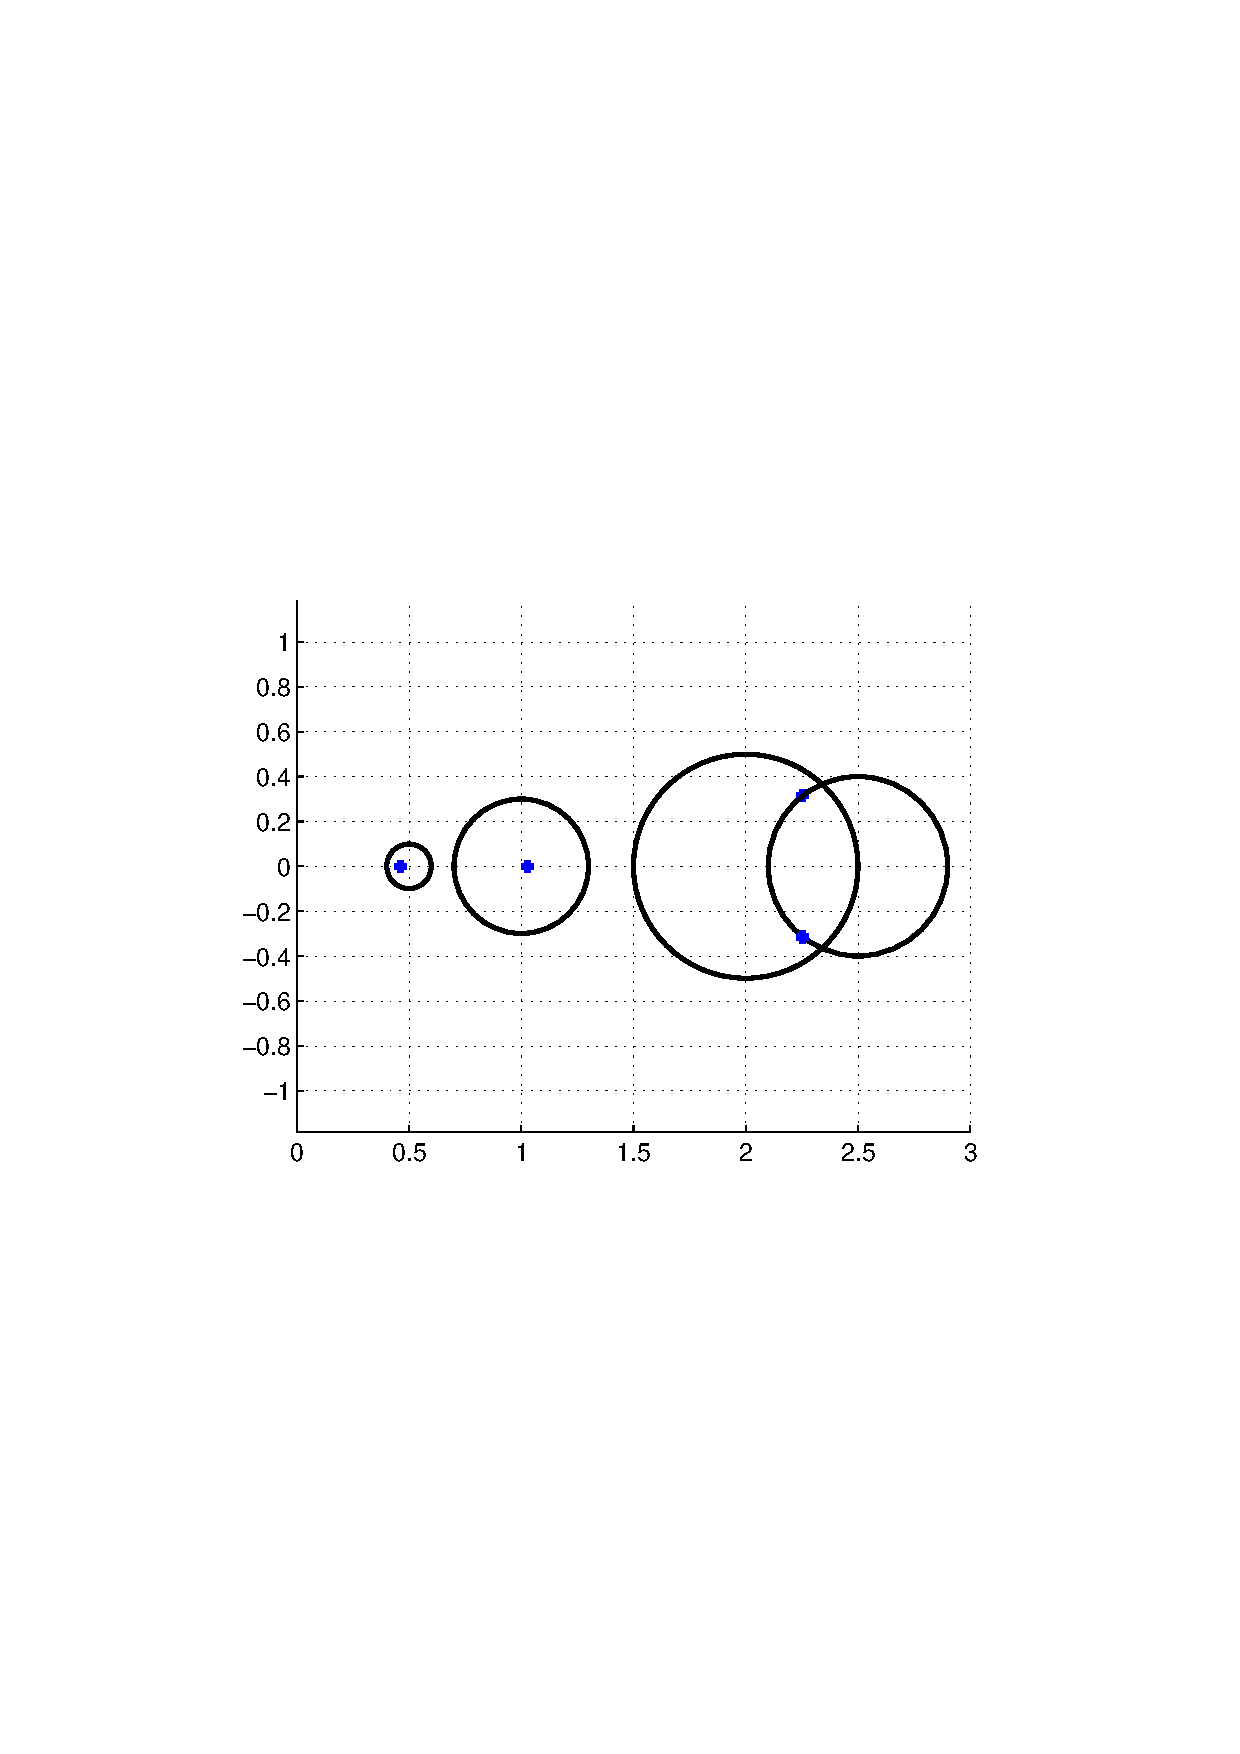
\includegraphics[width = \columnwidth]{gersh.pdf}
\end{minipage}

Sur cet exemple, les seuls disques qui contiennent deux valeurs propres sont
ceux qui s'intersectent. Les autres en contiennent une et une seule. Ce
phénomène, qui n'est pas anodin, est l'objet de l'exercice suivant.

\begin{exercice}
\label{ex:gersh} On note $\mathcal E$ une composante connexe de $\mathcal G(A)$ et $p$ le nombre de disques $D_i$ inclus dans $\mathcal E$. Ainsi, dans l'Exemple, $\mathcal G(A)$ a 3 composantes connexes
\begin{displaymath}
D_1 \ (p = 1),\quad D_2 \ (p = 1), \quad D_3 \cup D_4 \ (p= 2)
\end{displaymath}
Le but de l'exercice est de montrer que $\mathcal E$ contient exactement $p$
valeurs propres de $A$ (comptées avec leur ordre de multiplicité algébrique). 

A cet effet, on note $D$ la diagonale de $A$ et, pour tout $0 \leq r \leq 1$
\begin{displaymath}
A_r = rA + (1-r)D
\end{displaymath}
On note enfin $m(r)$ le nombre de valeurs propres de $A_r$ dans $\mathcal E$.
On cherche donc à montrer : $m(1) = p$.
\begin{enumerate}
\item Démontrez que $m(0) = p$.
\item Démontrez que $\mathcal G(A_r) \subset \mathcal G(A)$.
\item {Supposez qu'il existe} $\gamma$ une arc simple $\mathcal C^1$ par
	morceaux orienté positivement séparant $\mathcal E$ (à l'intérieur) de
	$\mathcal G(A) \setminus \mathcal E$ (à l'extérieur). Démontrez que
\begin{displaymath}
m(r) = \int_{\gamma} \frac{\chi'_{r}(z)}{\chi_{r}(z)}dz
\end{displaymath}
où $\chi_{r}$ est le polynôme caractéristique de $A_r$.
\item Déduisez que que $m$ est continue et concluez.
%\item \textbf{Application.} On suppose que les disques $D_i$ sont deux-à-deux disjoints. Montrer que $A$ est diagonalisable.
%{\item Proposer une configuration où un tel arc $\gamma$ n'existe pas. Comment peut-on conclure dans ce cas ?}
\end{enumerate}
\end{exercice}

Ce résultat donne des critères puissants:

\begin{corollary}
	Si les disques de Gershgorin d'une matrice sont deux-à-deux disjoints alors
	la matrice est diagonalisable.
\end{corollary}

\begin{corollary}
	Soit~$A$ une matrice irréductible et fortement diagonale dominante
	($\ \abs{a_{ii}}\ge\sum_{i\neq j}\abs{a_{ij}}$ avec au moins une inégalité
	stricte).  Alors~$A$ est inversible.
\end{corollary}

%Citons pour finir un résultat de  \cite{serre2001} sur le domaine de
%Gershgorin d'une matrice $A$ \emph{irréductible} : si une valeur propre est
%sur la frontière de $\mathcal G(A)$, c'est un point d'intersection de tous
%les cercles.
Citons enfin le
% théorème de Gauss-Lucas
\begin{exercice}[Théorème de Gauss-Lucas]
	Les racines d'un polynôme dérivé~$P'$ sont dans l'enveloppe convexe des
	racines de~$P$.
\end{exercice}

\paragraph{Éléments singuliers}
Les éléments propres sont définis seulement pour les matrices carrées.
Encore, les théorèmes les plus intéressants sur les éléments propres portent
seulement sur les matrices hermitiennes.  On peut résoudre tout à coup ces
deux contraintes en considérant la matrice~$A^*A$ associée à toute matrice
rectangulaire~$A\in\M_{p,q}(\K)$.  Observons que~$A^*A$ est carrée et
hermitienne, et par le théorème spectral elle diagonalise avec des valeurs
propres réels~$\ge 0$.

\begin{definition}
	Les \emph{valeurs singulières} d'une matrice~$A\in\M_{p,q}(\K)$ sont les
	valeurs propres de la matrice~$A^*A$.  On les
	écrit~$\sigma_i(A)=\lambda_i(A^*A)$ pour~$i=1,\ldots q$,
	typiquement par ordre décroissant~$\sigma_1\ge\cdots\ge\sigma_q$.
\end{definition}

\begin{proposition}
	\label{prp:singular}
	Les valeurs singulières d'une matrice sont toujours des nombres réels
	non-négatifs.  Le nombre de valeurs singulières différentes coïncide avec
	le rang de la matrice.  Pour une matrice hermitienne, les valeurs
	singulières sont ses valeurs propres en valeur absolue.
\end{proposition}

\begin{exercice}
	Démontrer la proposition~\ref{prp:singular}.
\end{exercice}

Plus tard, on verra que toute matrice~$A\in\M_{p,q}$ admet
une~\emph{décomposition en valeurs singulières} (SVD) de la forme~$A=U\Sigma V$,
où~$\Sigma\in\M_{p,q}(\R)$ est diagonale avec valeurs singulières de~$A$
sur sa diagonale, et les matrices~$U,V$ sont unitaires de taille~$p$ et~$q$
respectivement.


\subsection{Normes matricielles}

% def. norme matricielle

\begin{definition}[norme]
	Soit~$V$ un espace vectoriel sur~$\K$.
	Une~\emph{norme} sur~$V$ est une application~$p:V\to\R$
	qui satisfait les propriétés suivantes
	\begin{enumerate}
		\item[(i)] $p(\x) = 0\ \implies\ \x=0$
		\item[(ii)] $p(\x)\ge 0$
		\item[(iii)] $p(\x+\y)\le p(\x)+p(\y)$
		\item[(iv)] $p\parens{\lambda\x}=\abs{\lambda}p(\x)$
	\end{enumerate}
	Si toutes les propriétés sont satisfaites sauf (i) on dit que~$p$
	est une~\emph{seminorme}.
\end{definition}

\begin{definition}[norme matricielle]
	Une~\emph{norme matricielle} sur les matrices carrées de dimension~$n$ est
	une application~$p:\M_n(\K)\to\R$ telle que
	\begin{enumerate}
		\item[(i)] $p$ est une norme sur l'espace vectoriel~$\M_n(\K)$
		\item[(ii)] $p(AB) \le p(A) p(B)$
	\end{enumerate}
\end{definition}

L'espace vectoriel~$\M_n(\K)$ est de dimension finie donc toutes les normes
sont équivalentes.  Ceci est très pratique : pour démontrer la convergence
d'une suite de matrices, il suffit de le faire avec la norme pour laquelle la
démonstration est plus facile.  Voyons quelques exemples de normes
matricielles.

% def. norme induite / norme d'opérateur , lemme de composition

\begin{definition}[norme induite]
	Soit~$\Abs\cdot$ une norme en~$\K^n$.  La~\emph{norme induite}
	par~$\Abs\cdot$ sur~$\M_n(\K)$ est la norme de l'opérateur
	linéaire %~$\K^n\to\K^n$
	associé à chaque matrice, notée~$\ABS\cdot$.  Ainsi
	\[
		\ABS{A}
		=
		\sup_{\x\neq0}\frac{\Abs{A\x}}{\Abs\x}
		=
		\max_{\Abs\x=1}\Abs{A\x}
	\]
	La norme induite par la norme~$\Abs\cdot_p$ de~$\K^n$
	s'écrit~$\ABS\cdot_p$.
\end{definition}

\begin{exercice}
	Démontrez que toute norme induite est une norme matricielle, et qu'elle
	satisfait les deux propriétés suivantes
	\begin{enumerate}
		\item[(i)] $\Abs{A\x}\le\ABS A\cdot\Abs\x$
		\item[(ii)] $\ABS I = 1$
	\end{enumerate}
\end{exercice}

\begin{exercice}
	Démontrez que la~\emph{norme de Frobenius} définie par
	\[
		\ABS A_F
		=
		\sqrt{\mathrm{tr}\parens{A^*A}}
		=
		\sqrt{\sum_{i,j}\Abs{a_{ij}}^2}
	\]
	est une norme matricielle mais n'est pas une norme induite.
\end{exercice}

% normes induites par la norme p=1,2,\infty

\begin{exercice}
	Vérifiez les caractérisations suivantes des normes induites classiques:
	\[
		\ABS A_1      = \max_j\sum_i\abs{a_{ij}}
		\qquad
		\ABS A_\infty = \max_i\sum_j\abs{a_{ij}} = \ABS{A^*}_1
		\qquad
		\ABS A_2      = \sqrt{\rho\parens{A^*A}} = \ABS{A^*}_2
	\]
\end{exercice}

% lien entre normes induites et rayon spectral

\begin{exercice}[Lien entre normes induites et rayon spectral]
	Démontrez que %les affirmations suivantes:
	\begin{enumerate}
		\item Pour toute matrice~$A\in\M_n(\K)$ on
			a~$\rho\parens{A^m}=\rho\parens{A}^m$ et~$\rho\parens{\lambda
			A}=\abs\lambda\rho\parens{A}$
		\item Si~$A$ est diagonale alors~$\ABS A_p=\rho(A)$
			pour~$1\le p\le\infty$.
		\item Si~$A$ est normale alors~$\ABS A_2=\rho(A)$.
		\item Si~$n>1$ alors le rayon spectral~$\rho$ n'est pas une norme
			sur~$\M_n(\K)$.
		\item Si~$\ABS\cdot$ est une norme induite sur~$\M_n(\C)$ alors
			\begin{equation}\label{eq:rholessthanABS}
				\rho(A)\le\ABS A
			\end{equation}
		\item${}^*$ L'équation~(\ref{eq:rholessthanABS}) est encore vraie pour
			une norme matricielle quelconque sur~$\M_n(\C)$, ou même
			sur~$\M_n(\R)$.
	\end{enumerate}
\end{exercice}

% théorème de Householder

L'inégalité~\ref{eq:rholessthanABS} dit que~$\rho(A)$ minore
l'ensemble~$\left\{\ABS A\ :\ \ABS\cdot\ \textrm{norme induite}\right\}$.  Le
théorème de Householder montre que c'est en fait la borne inférieure

\begin{theorem}[Householder]
	Pour toute matrice~$A\in\M_n(\C)$ et tout~$\epsilon>0$ il existe une norme
	induite~$\ABS\cdot_{A,\epsilon}$ telle que
	\begin{equation}\label{eq:rholessthanABS}
		\ABS A_{A,\epsilon}\le\rho(A)+\epsilon
	\end{equation}
\end{theorem}

\begin{exercice}[Démonstration du théorème de Householder]$ $
	\begin{enumerate}
		\item Soit~$\Abs\cdot_\alpha$ une norme en~$\K^n$ et~$P\in GL_n(\K)$.
			Démontrez que~$N(\x)=\Abs{P\x}_\alpha$ est une norme en~$\K^n$ et que
			sa norme induite est~$N(A)=\ABS{PAP^{-1}}_\alpha$.
		\item Soit~$A\in\M_n(\C)$ et~$\mu>0$, démontrez qu'il existe~$Q\in
			GL_n(\C)$ et~$D$ diagonale telles que~$Q^{-1}AQ=D+\OO(\mu)$
		\item Démontrez le théorème de Householder.
	\end{enumerate}
\end{exercice}


% convergence de suites de matrices
%% \sum A^n  est convergente (vers 0) sii rho(A) < 1 et alors I-A est inversible
%% rho(A) = \lim |||A^n|||^(1/n)
%% exponentielle d'une matrice

\begin{exercice}[Convergence de suites de matrices]
	Démontrez les propositions suivantes:
	\begin{enumerate}
		\item Pour une norme induite, la condition~$\ABS A<1$ implique que~$I-A$
			est inversible, et l'inverse est la somme de la série
			normalement convergente~$\ds\sum_{k\ge0}A^k$.
		\item Pour toute matrice~$A\in\M_n(\K)$, la
			série~$\ds\sum_{k\ge0}\tfrac1{k!}A^k$ est normalement convergente.
			Sa limite~$e^A$ est une matrice inversible.
		\item $*$ Pour toute norme induite, on a
			toujours~$\ds\rho(A)=\lim_{k\to\infty}\ABS{A^k}^{\frac1k}$
	\end{enumerate}
\end{exercice}


\subsection{Conditionnement de matrices}

Beaucoup de problèmes de modélisation se réduisent à la solution de
l'équation~$Ax=b$.  L'opérateur~$A$ représente un système physique agissant
sur un état~$x$ que l'on veut connaître, et~$b$ est l'observation faite.
Dû à des erreurs de mesure, le vecteur~$b$ est souvent perturbé par le bruit,
ce qui donnera une valeur~$x$ inexacte.

{\bf Exemple.} (issu de [AK], section 5.3)
\begin{displaymath}
A = \left(\begin{array}{cccc}
8 & 6 & 4 & 1 \\
1 & 4 & 5 & 1 \\
8 & 4 & 1 & 1 \\
1 & 4 & 3 & 6
\end{array}\right), \quad b =  \begin{pmatrix}8 \\ 10 \\ 2 \\ 6\end{pmatrix} \quad
\Rightarrow \quad
x = \begin{pmatrix}0 \\ 0 \\ 2 \\ 0\end{pmatrix}
\end{displaymath}
En modifiant légèrement~$b$, on obtient une solution très différente
\begin{displaymath}
A = \left(\begin{array}{cccc}
8 & 6 & 4 & 1 \\
1 & 4 & 5 & 1 \\
8 & 4 & 1 & 1 \\
1 & 4 & 3 & 6
\end{array}\right), \quad b = \begin{pmatrix}8.05 \\ 10 \\ 2 \\ 6\end{pmatrix} \quad
\Rightarrow \quad x = \begin{pmatrix}2 \\ -5.225 \\ 5.5 \\ 1.4\end{pmatrix}
\end{displaymath}

Le~\emph{conditionnement} d'une matrice sert à étudier cet effet.

\begin{definition}[conditionnement d'une matrice]
	Soit~$A$ une matrice inversible et~$\ABS\cdot_\alpha$ une norme induite.  Le
	\emph{conditionnement} de~$A$ relatif à cette norme est
	\[
		\mathrm{cond}_\alpha(A) = \ABS A\ABS{A^{-1}}
	\]
\end{definition}

\begin{proposition}[conditionnement euclidien] Pour toute matrice
	inversible~$A$:
\begin{displaymath}
\mathrm{cond}_2(A) = \sqrt{\frac{\lambda_{\max}(A^*A)}{\lambda_{\min}(A^*A)}}
\end{displaymath}
Si $A$ est normale
\begin{displaymath}
\mathrm{cond}_2(A) = \frac{\abs{\lambda_{\max}(A)}}{\abs{\lambda_{\min}(A)}}
\end{displaymath}
Si $O \in U_n(\K)$ alors
\begin{displaymath}
\mathrm{cond}_2(O) = 1, \quad \mathrm{cond}_2(AO) = \mathrm{cond}_2(OA) = \mathrm{cond}_2(A)
\end{displaymath}
\end{proposition}

%Les deux exercices suivants montrent que, lorsqu'on résout un problème de la
%forme~$Ax=b$, le conditionnement de~$A$ sert à majorer l'erreur de la
%solution à partir du bruit sur~$b$ ou même sur~$A$:
%\clearpage
Lorsqu'on résout un problème de la forme~$Ax=b$, le conditionnement de~$A$
sert à majorer l'erreur relatif de la solution~$x$.  On présente deux
versions de cette majoration, selon si on a des petites erreurs d'observation
(sur~$b$) ou de modélisation (sur~$A$):

\begin{exercice}[effet des erreurs d'observation]
	Soit~$\delta b$ une perturbation du second membre et~$\delta x$ l'erreur
	induit sur la solution, de sorte que~$A(x+\delta x)=b+\delta b$.  Démontrez
	que l'erreur relatif augmente d'un facteur au plus~$\mathrm{cond}(A)$:
	\[
		\frac{\Abs{\delta x}}{\Abs{x}}
		\le
		\mathrm{cond}(A)
		\frac{\Abs{\delta b}}{\Abs{b}}
	\]
	Démontrez que cette inégalité est optimale: il existe~$b$ et~$\delta
	b$ tels que l'égalité a lieu.
\end{exercice}


\begin{exercice}[effet des erreurs de modélisation]
	Soit~$\delta A$ une perturbation de la matrice et~$\delta x$ l'erreur
	induit sur la solution, de sorte que~$(A+\delta A)(x+\delta x)=b$.  Démontrez
	que l'erreur relatif augmente d'un facteur au plus~$\mathrm{cond}(A)$:
	\[
		\frac{\Abs{\delta x}}{\Abs{x+\delta x}}
		\le
		\mathrm{cond}(A)
		\frac{\ABS{\delta A}}{\ABS{A}}
	\]
	Démontrez que cette inégalité est optimale: il existe~$b$ et~$\delta
	A$ tels que l'égalité a lieu.
\end{exercice}

\begin{remark}
	D'après ces exercices, il est préférable que le conditionnement de $A$ soit
	proche de 1. Ceci est d'autant plus vrai pour les méthodes itératives où
	les erreurs sont propagées et amplifiées à chaque itération. La technique
	du \emph{préconditionnement} consiste à considérer un système linéaire
	équivalent
	\[
		PAx = Pb
	\]
	où la matrice~$P$, dite le~\emph{préconditionneur} a été choisie de façon
	que $\mathrm{cond} (PA) < \mathrm{cond}(A)$. Il existe plusieurs méthodes
	pour bien choisir $P$, par exemple si~$A$ est à diagonale dominante on peut
	choisir~$P=\mathrm{diag}(A)^{-1}$.
	On pourra consulter à ce sujet [AK, Chapitre 5].
\end{remark}

\begin{remark}
\label{rm:cond}
Les inégalités ci-dessus sont certes optimales, mais elles sont en général
très pessimistes (on dit aussi \emph{conservatives}). Ainsi dans
l'Exemple on a
\begin{displaymath}
\frac{\Abs{\delta x}_{2}}{\Abs{x}{2}} \simeq 964 \frac{\Abs{\delta
b}_{2}}{\Abs{b}_{2}}
\end{displaymath}
ce qui fait déjà beaucoup, mais $\mathrm{cond}_2(A) \simeq 3199$.
\end{remark}

{\bf Exemple avec le laplacien 1D.}

On définit la matrice symétrique suivante, dite le <<laplacien discret 1D>>:
%(discrétisation par différences finies de la dérivée seconde):
\begin{equation}
\label{eq:A}
A = n^2 \left(\begin{array}{cccc}
2 & -1 & &  \\
-1 & \ddots & \ddots & \\
  & \ddots & \ddots & -1 \\
 & & -1 & 2
\end{array}\right) \in M_{n-1}(\R)
\end{equation}
Cette matrice apparait de manière naturelle quand on discrétise l'équation de
Laplace en dimension~$1$ (avec conditions de Dirichlet):
\begin{equation*}
	\begin{cases}
		u''(x)  = -f(x) & 0 < x < 1 \\
		u(x) = 0 & x\in\{0,1\}
\end{cases}
\end{equation*}
On fixe~$n\ge 1$ et on note
\begin{displaymath}
	x_i = \frac{i}{n}, \quad 0 \leq i \leq n, \quad U = \begin{pmatrix}u(x_1)
		\\ \vdots \\ u(x_{n-1})\end{pmatrix} \in \R^{n-1}, \quad  b =
		\begin{pmatrix}f(x_1) \\ \vdots \\ f(x_{n-1})\end{pmatrix} \in \R^{n-1}
\end{displaymath}
Le problème discret est donc~$Ax=b$, avec une solution qui devrait
s'approcher de~$U$ (pour cela on va supposer que~$f$ est suffisamment
régulière).


\begin{exercice}[étude du Laplacien 1D]$ $
	\begin{enumerate}
		\item Démontrez que~$AU=b+\mathcal{O}\parens{\frac1{n^2}}$
		\item Démontrez que les valeurs propres de~$A$ sont $$\lambda_k = 4n^2
			\sin^2 \frac{\alpha_k}{2}, \quad \alpha_k =  \frac{k \pi}{n}, \quad
			1\leq k \leq n-1$$ avec pour vecteur propre associé $v_k = (\sin j
			\alpha_k)_{1 \leq j \leq n-1}$.\\
			Pouvait-on voir autrement que $A \in S_{n-1}^{++}(\R)$ ?
		\item Soit~$U_{\mathrm{approx}}$ la solution du système linéaire~$Ax=b$.
			Démontrez
			que $\Abs{U-U_{\mathrm{approx}}}_2=\mathcal{O}\parens{\frac1{n^2}}$
\item Démontrez que
\begin{displaymath}
	\mathrm{cond}_2(A) \underset{n \rightarrow \infty}{\sim} \frac{4n^2}{\pi^2}
\end{displaymath}
de sorte que, quand $n$ est grand, la matrice est très mal conditionnée.
\item En notant $\x = U_{\mathrm{approx}}$, montrer que
\begin{displaymath}
\lim_{n \rightarrow \infty } \frac{1}{n} \Abs{\x}^2 = \int_0^1 u^2(x)dx,
\quad \lim_{n \rightarrow \infty } \frac{1}{n} \Abs{b}^2 = \int_0^1 f^2(x)dx
\end{displaymath}
	\end{enumerate}
\item Montrer enfin qu'il existe une constante $c > 0$ indépendante de $n$ telle que
\begin{displaymath}
\frac{\Abs{\delta\x}}{\Abs{\x}} \leq c \frac{\Abs{\delta b}}{\Abs{b}}
\end{displaymath}
de sorte que, même si la matrice est très mal conditionné, le problème est
très bien posé pour les conditions d'utilisation typiques.
\end{exercice}

%\begin{exercice}
%On va analyser la matrice $A$ du Laplacien discrétisé à la lumière de cette
%remarque.
%\begin{enumerate}
%\item Montrer que 
%\begin{displaymath}
%	\mathrm{cond}_2(A) \underset{n \rightarrow \infty}{\sim} \frac{4n^2}{\pi^2}
%\end{displaymath}
%de sorte que, quand $n$ est grand, la matrice est très mal conditionnée.
%\item En notant $x = U_{\textrm{approx}}$, montrer que
%\begin{displaymath}
%\lim_{n \rightarrow \infty } \frac{1}{n} \n{\xx}{2}^2 = \int_0^1 u^2(x)dx, \quad \lim_{n \rightarrow \infty } \frac{1}{n} \n{b}{2}^2 = \int_0^1 f^2(x)dx
%\end{displaymath}
%\item Montrer enfin qu'il existe une constante $c > 0$ indépendante de $n$ telle que
%\begin{displaymath}
%\frac{\n{\delta x}{2}}{\n{\xx}{2}} \leq c \frac{\n{\delta b}{2}}{\n{b}{2}}
%\end{displaymath}
%\end{enumerate}
%\end{exercice}


% exemple de mauvais conditionnement

% exemple 2 (matrice de Hilbert)

% déf. nombre de condition (associé à une norme induite)

% prop. exemples de cond2 à partir des rayons spectraux

% perturbation de x selon la perturbation de b (lors de la solution de Ax=b)

% perturbation de x selon la perturbation de A (lors de la solution de Ax=b)

% observation que les inégalités sont ``pessimistes''

% exemple de la dérivée seconde discrète


%\subsection{Exemples de problèmes linéaires}
%
%\subsection{Analyse matricielle}
%
%- groupes de matrices
%
%- théorème spéctral
%
%- rayon spéctral
%
%- normes matricielles
%
%- normes induites
%
%- théorème de Householder
%
%- conditionnement d'une matrice: définition, propriétés, exemple du laplacien
%à 5 points


\end{document}
\clearpage
\section{Factorisation de matrices}

\subsection{Systèmes triangulaires et élimination gaussienne}

\subsection{Factorisation LU}

\subsection{Factorisation de Cholesky}

\subsection{Factorisation QR}

%\section{Décomposition de matrices}

\subsection{Diagonalisation}

\subsection{Décomposition polaire}

\subsection{Décomposition SVD}

\subsection{Décomposition SVD incomplète}


\section{Méthodes itératives}

\subsection{Méthodes itératives de résolution: formulation générale}

\subsection{Méthodes de Jacobi et Gauss-Seidel}

\subsection{Descente de gradient à pas fixe}

\subsection{Descente de gradient à pas optimal}

\subsection{Descente de gradient stochastique}

\subsection{Méthode du gradient conjugué}

\subsection{Méthode de la puissance, puissance inverse}

\subsection{Méthodes de calcul de la SVD}

- bidiagonalisation + méthode itérative

%\subsection{Méthode QR}



\section{Éléments propres et singuliers}

\subsection{Exemples de problèmes de valeurs propres}

- polynômes (et matrice compagnon)

- acp

- analyse quantitative d'une EDO

- oscillations

- spectre d'un corps

\subsection{Valeurs singuliers}

- caractérisation variationnelle des valeurs propres et valeurs singuliers

\subsection{Analyse du spectre}


%\begin{verbatim}
%S4. Algèbre linéaire numérique : généralités
%4.0. Les 4 problèmes de l'algèbre linéaire selon Strang (Ax=b avec
%m=n, m<n, m>n, et Ax=lambda * x)
%4.1. Exemples de problèmes linéaires: minimisation quadratique,
%regression linéaire, EDO et EDP discrètes, splines
%4.2. Analyse matricielle: rayon spéctral, normes, normes induites,
%théorème de Householder
%
%S5. Algèbre linéaire numérique : méthodes de résolution
%5.1. Systèmes triangulaires, Algorithme d'élimination gaussienne
%5.2. Factorisation LU
%5.3. Factorisation Cholesky
%5.4. Méthodes iteratives : formulation générale
%5.5. Jacobi, Gauss-Seidel
%5.6. Gradient, gradient à pas optimal
%5.7. Conditionnement d'une matrice : définition, propriét'es, exemple
%pour le laplacien à 5 points
%
%S6. Algèbre linéaire numérique : éléments propres
%6.1. Exemples de problèmes de valeurs propres : ACP, analyse
%quantitative d'une EDO, oscillations, polynômes
%6.2. Analyse du spectre: cercles de Gershgorin, Gauss-Lucas
%6.3. Méthode de la puissance, puissance inverse
%6.4. Décomposition QR : existence, unicité, algorithmes
%
%S7. Résolution d'équations non-linéaires
%7.1. Méthodes en dimension 1: bisection, Newton, secante
%7.2. Racines de polynomes d'une variable
%7.3. Cas vectoriel: optimisation vs résolution d'une équation (
%min{F(x)} vs F'(x)=0 ), rappel des multiplicateurs de Lagrange
%7.4. Méthode de Newton et variantes
%\end{verbatim}

% vim:set tw=77 filetype=tex spell spelllang=fr ts=2 sw=2:

